\documentclass[conference]{IEEEtran}
\IEEEoverridecommandlockouts

\usepackage{cite}
\usepackage{amsmath,amssymb,amsfonts}
\usepackage{graphicx}
\usepackage{textcomp}
\usepackage{booktabs}
\usepackage{multirow}
\usepackage{xcolor}
\usepackage{url}
\usepackage{hyperref}
\hypersetup{colorlinks=true,linkcolor=blue,citecolor=blue,urlcolor=blue}

\begin{document}

\title{Uncertainty-Gated Test-Time Adaptation for Reliable\\
Cross-Hospital Histopathology Classification}

\author{
\IEEEauthorblockN{Anonymous authors}
\IEEEauthorblockA{Paper under double-blind review.\\
Short name: UTTA-Med}
}

\maketitle

\begin{abstract}
Models trained on histopathology patches from source hospitals degrade on an unseen hospital.
Test-time adaptation (TTA) can recover some of that drop, but entropy minimization on every target sample can also amplify errors.
We ask whether restricting TTA to low-uncertainty samples makes adaptation safer under real Camelyon17-WILDS shift (source hospitals $\{0,3,4\}$ $\rightarrow$ target hospital $2$).
We train ResNet-18 source models on five seeds and compare source-only, Tent, EATA, and four gates---random, softmax confidence, predictive entropy, and MC-Dropout variance---under a frozen protocol: BatchNorm affine updates only, running statistics frozen, TTA learning rate $10^{-5}$, and gate thresholds chosen on hospital~1.
On hospital~2, source AUROC is $0.930\pm0.009$.
Fair Tent is unstable: it collapses on $2/5$ seeds (mean AUROC $0.698\pm0.324$, harm rate $0.187\pm0.179$).
Selective gates never collapse, raise F1 on all five seeds, and cut harm to $0.007\pm0.003$.
UTTA-Med (MC-Dropout) does \emph{not} outperform softmax confidence ($\Delta$~AUROC $<0.001$ on every seed).
Random gating also collapses on $2/5$ seeds, so the benefit is \emph{which} samples are used, not merely using fewer of them.
Under this binary protocol, gating is what makes TTA reliable; MC-Dropout is a valid error signal but is redundant with confidence.
\end{abstract}

\begin{IEEEkeywords}
Test-time adaptation, uncertainty, MC-Dropout, histopathology, Camelyon17, calibration, harmful adaptation
\end{IEEEkeywords}

\section{Introduction}

A classifier trained on labeled patches from source hospitals is often deployed on a new scanner, stain, and patient population.
Formally $P_{\mathrm{source}}(X,Y)\neq P_{\mathrm{target}}(X,Y)$.
Test-time adaptation (TTA) updates a frozen source checkpoint using unlabeled target images, typically by entropy minimization on BatchNorm affine parameters~\cite{wang2021tent}.
The known failure mode is \emph{harmful adaptation}: a wrong prediction becomes an update signal and the model degrades.

We study a hard gate: adapt only if predictive uncertainty $U(x)<\tau$, otherwise skip the sample.
UTTA-Med estimates $U(x)$ by Monte Carlo Dropout variance~\cite{gal2016dropout}.
We do \textbf{not} claim the first uncertainty-aware TTA method.
Closest prior work includes EATA (entropy + diversity filtering)~\cite{niu2022eata} and SAR (sharpness-aware TTA)~\cite{niu2023sar}.
Our difference is (i)~an explicit MC-Dropout \emph{variance} gate, (ii)~matched-coverage controls against random, confidence, and entropy gates, and (iii)~joint reporting of coverage, harm rate, and calibration on a leakage-controlled Camelyon17-WILDS split~\cite{koh2021wilds,bandi2018camelyon17}.

\textbf{Contributions.}
(1)~A frozen, leakage-free Camelyon17 TTA protocol (official hospitals; target labels unused until the final test pass).
(2)~Evidence that ungated Tent is unstable even with conservative BN-affine updates (collapse on $2/5$ seeds).
(3)~Evidence that selective TTA prevents collapse, cuts harm $\sim$25$\times$ vs.\ Tent, and improves F1 on $5/5$ seeds.
(4)~A negative-but-informative control: MC-Dropout $\approx$ softmax confidence for this binary ResNet-18.

\section{Related work}

Tent~\cite{wang2021tent} minimizes prediction entropy at test time, updating BatchNorm affine parameters.
EATA~\cite{niu2022eata} filters high-entropy samples and reweights by diversity; EATA-C additionally uses a calibration-style entropy threshold.
SAR~\cite{niu2023sar} uses sharpness-aware optimization and removes very high-entropy samples from the loss.
Several medical TTA papers use entropy or confidence filters; we do not claim primacy.

UTTA-Med uses stochastic predictive \emph{variance} as a hard participation gate and evaluates that gate against random / confidence / entropy at matched validation coverage.
EATA is kept as a published-style baseline under the \emph{same} BN-affine update scope so that filtering strategy is not confounded with which parameters move.
We restrict SAR to optional follow-up: its optimizer is a second axis of variation.

\section{Method}

\subsection{Data and leakage}
Camelyon17-WILDS~\cite{koh2021wilds} provides $96\times96$ RGB patches and a binary tumor/non-tumor label based on the central $32\times32$ region.
Hospital IDs were read from the official loader (HuggingFace parquet dump of WILDS), never hard-coded from secondary documents.

\begin{table}[t]
\centering
\caption{Official split used throughout. Hospital~1 is for $\tau$ and early stopping only. Hospital~2 labels are touched once, after those choices are frozen.}
\label{tab:splits}
\small
\begin{tabular}{@{}lccc@{}}
\toprule
Role & Hospitals & Patches & WSIs \\
\midrule
Source train & 0, 3, 4 & 302{,}436 & 30 \\
In-domain val & 0, 3, 4 & 33{,}560 & 30$^\dagger$ \\
OOD val (tune) & \textbf{1} & 34{,}904 & 10 \\
Target test & \textbf{2} & 85{,}054 & 10 \\
\bottomrule
\end{tabular}\\[2pt]
{\scriptsize $^\dagger$Same source slides, held-out patches. Train $\cap$ OOD-val slides $=\emptyset$, train $\cap$ test $=\emptyset$, OOD-val $\cap$ test $=\emptyset$.}
\end{table}

\subsection{Source model}
ResNet-18~\cite{he2016resnet} (ImageNet initialization), global average pooling, head Linear--ReLU--Dropout($0.5$)--Linear with \textbf{one logit}, trained with BCE-with-logits.
Adam $10^{-4}$, batch $128$, at most $20$ epochs, patience $5$ on hospital-1 AUROC, save-best-only.
Seeds $\{42,123,2024,7,99\}$.

\subsection{TTA protocol (all methods)}
Continual one pass over the target stream (\texttt{shuffle=False}), one Adam step per batch.
Only BatchNorm $\gamma,\beta$ are trainable; running mean/variance are \textbf{frozen}.
TTA learning rate $10^{-5}$ was selected on hospital~1 after $\{10^{-4},2.5\cdot10^{-4},10^{-3}\}$ collapsed Tent.
If a gated batch has zero accepted samples, we skip \texttt{backward()} and \texttt{step()} (no $\varepsilon$-smoothed denominator).

\subsection{UTTA-Med gate}
Dropout remains active.
$N=20$ stochastic forward passes:
\begin{equation}
\bar p(x)=\frac1N\sum_{j=1}^N p_j,\qquad
U(x)=\frac1N\sum_{j=1}^N \bigl(p_j-\bar p\bigr)^2.
\end{equation}
\begin{equation}
w(x)=\mathbf{1}\bigl[U(x)<\tau\bigr],\qquad
L=\frac{\sum_i w_i\,H(p_i)}{\sum_i w_i}
\end{equation}
if $\sum_i w_i>0$, else skip the batch.
$\tau$ is the \textbf{70th percentile} of $U$ on hospital~1.
The percentile \emph{rule} is frozen after seed~42; the numeric $\tau$ is re-estimated per seed.

\subsection{Controls}
\textbf{Tent:} $w\equiv 1$.
\textbf{EATA:} entropy margin $e=0.4$, same BN-affine scope.
\textbf{Random:} each sample is adapted with probability equal to UTTA coverage on hospital~1 ($\approx 0.70$).
\textbf{Confidence:} adapt if $\max(p,1-p)\ge t$, with $t$ set to matched coverage on hospital~1.
\textbf{Entropy:} adapt if $H(p)\le t_H$, matched the same way.
For a Bernoulli probability, $H(p)$ is a strictly monotone function of $\max(p,1-p)$, so entropy and confidence gates are expected to coincide. They did, on every seed.

Harm rate is
$(C\!\to\!W)/C_{\mathrm{before}}$;
correction rate is
$(W\!\to\!C)/W_{\mathrm{before}}$.
Coverage is $N_{\mathrm{accepted}}/N_{\mathrm{target}}$, reported for every gated method.

\section{Results}

All test numbers are hospital~2, seeds $\{42,123,2024,7,99\}$.
Target labels were not used for training, $\tau$, or model selection.

\subsection{RQ1: Shift is real}
In-domain AUROC is $\approx 0.999$.
Target source-only AUROC is $\mathbf{0.930\pm0.009}$ (drop $0.070\pm0.009$).
F1 drop is larger ($0.18\pm0.02$): the source model becomes under-sensitive on the unseen hospital (typical recall $0.64$--$0.75$ vs.\ specificity $>0.95$).

\subsection{RQ3: Uncertainty tracks error}
On hospital~1, before any gating, MC-Dropout $U$ increases monotonically with error on all five seeds (Pearson $r=0.397\pm0.016$).
Lowest-uncertainty decile error $\approx 0\%$; highest-decile error $35$--$42\%$ (Fig.~\ref{fig:uerror}).
The uncertainty signal is informative; gating is justified.

\begin{figure}[t]
\centering
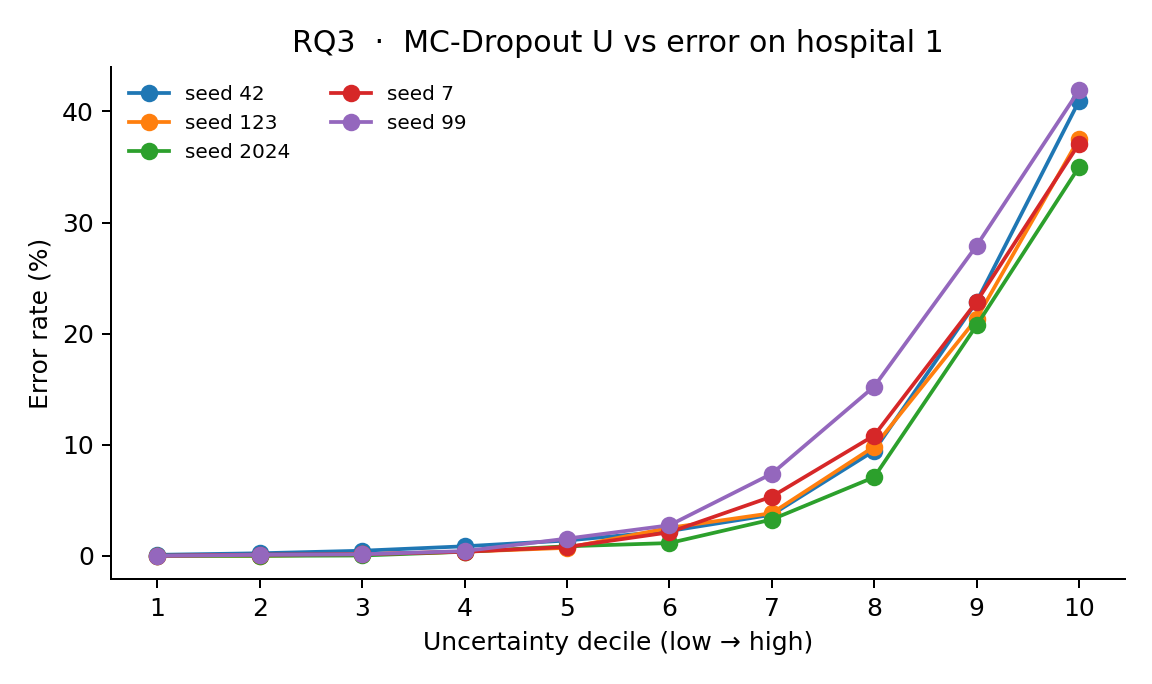
\includegraphics[width=\columnwidth]{figs/fig_u_error.png}
\caption{MC-Dropout uncertainty vs.\ error on hospital~1 (five seeds). Decile~1 error $\approx 0\%$; decile~10 $\approx 35$--$42\%$. $r=0.40\pm0.02$.}
\label{fig:uerror}
\end{figure}

\subsection{RQ2/RQ4: Ungated TTA is unsafe; gating is not ``fewer samples''}
\begin{table*}[t]
\centering
\caption{Hospital~2, mean $\pm$ std over five seeds. Entropy $\equiv$ confidence (binary). Harm $=$ fraction of previously correct patches flipped wrong.}
\label{tab:main}
\small
\begin{tabular}{@{}lccccc@{}}
\toprule
Method & AUROC & F1 & ECE & Harm & Cov. \\
\midrule
Source-only & $0.930\pm0.009$ & $0.807\pm0.025$ & $0.128\pm0.026$ & --- & --- \\
Tent & $0.698\pm0.324$ & $0.506\pm0.411$ & $0.284\pm0.179$ & $0.187\pm0.179$ & $1.00$ \\
EATA & $0.921\pm0.026$ & $0.809\pm0.031$ & $0.152\pm0.024$ & $0.025\pm0.015$ & $0.89$ \\
Random gate & $0.697\pm0.304$ & $0.487\pm0.385$ & $0.298\pm0.166$ & $0.194\pm0.170$ & $0.70$ \\
Confidence gate & $\mathbf{0.936\pm0.022}$ & $\mathbf{0.831\pm0.032}$ & $0.130\pm0.030$ & $\mathbf{0.007\pm0.003}$ & $0.58$ \\
UTTA-Med & $0.935\pm0.022$ & $0.830\pm0.032$ & $0.131\pm0.031$ & $0.007\pm0.003$ & $0.58$ \\
\bottomrule
\end{tabular}
\end{table*}

\begin{table}[t]
\centering
\caption{Per-seed hospital-2 AUROC. Bold: collapse ($<0.40$).}
\label{tab:perseed}
\small
\begin{tabular}{@{}lccccc@{}}
\toprule
Method & 42 & 123 & 2024 & 7 & 99 \\
\midrule
Source & 0.935 & 0.935 & 0.932 & 0.913 & 0.933 \\
Tent & 0.929 & 0.941 & 0.933 & \textbf{0.343} & \textbf{0.344} \\
EATA & 0.936 & 0.940 & 0.932 & 0.877 & 0.920 \\
Random & 0.922 & 0.937 & 0.897 & \textbf{0.354} & \textbf{0.373} \\
Confidence & 0.951 & 0.942 & 0.956 & 0.902 & 0.927 \\
UTTA-Med & 0.951 & 0.942 & 0.955 & 0.902 & 0.928 \\
\bottomrule
\end{tabular}
\end{table}

Tent with the conservative protocol still \textbf{collapsed on seeds 7 and 99} (AUROC $0.34$, F1 $0.05$, harm $\approx 0.38$; Table~\ref{tab:perseed}, Fig.~\ref{fig:perseed}).
On the other three seeds Tent is roughly source-level.
Mean Tent AUROC is therefore not a point estimate of a stable method; it is a mixture of ``fine'' and ``destroyed''.
EATA never collapsed but did not beat source AUROC.

Selective gates \textbf{never collapsed}.
Harm fell from $0.187$ (Tent) to $0.007$ (confidence / UTTA; Fig.~\ref{fig:harm}).
Random gating at $70\%$ coverage collapsed on the same two seeds as Tent: reducing the number of updates is not sufficient.

\begin{figure}[t]
\centering
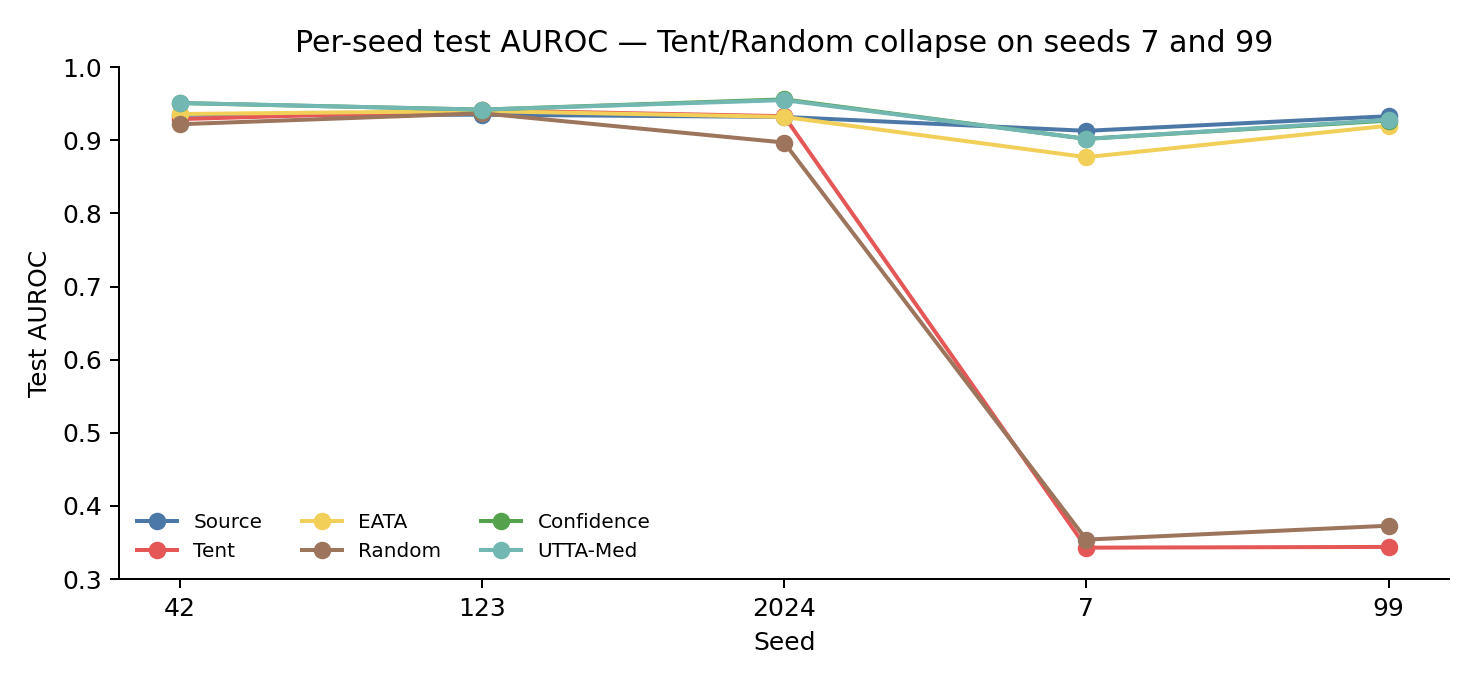
\includegraphics[width=\columnwidth]{figs/fig_per_seed.png}
\caption{Per-seed hospital-2 AUROC. Tent and random collapse on seeds 7 and 99; confidence and UTTA-Med do not.}
\label{fig:perseed}
\end{figure}

\begin{figure}[t]
\centering
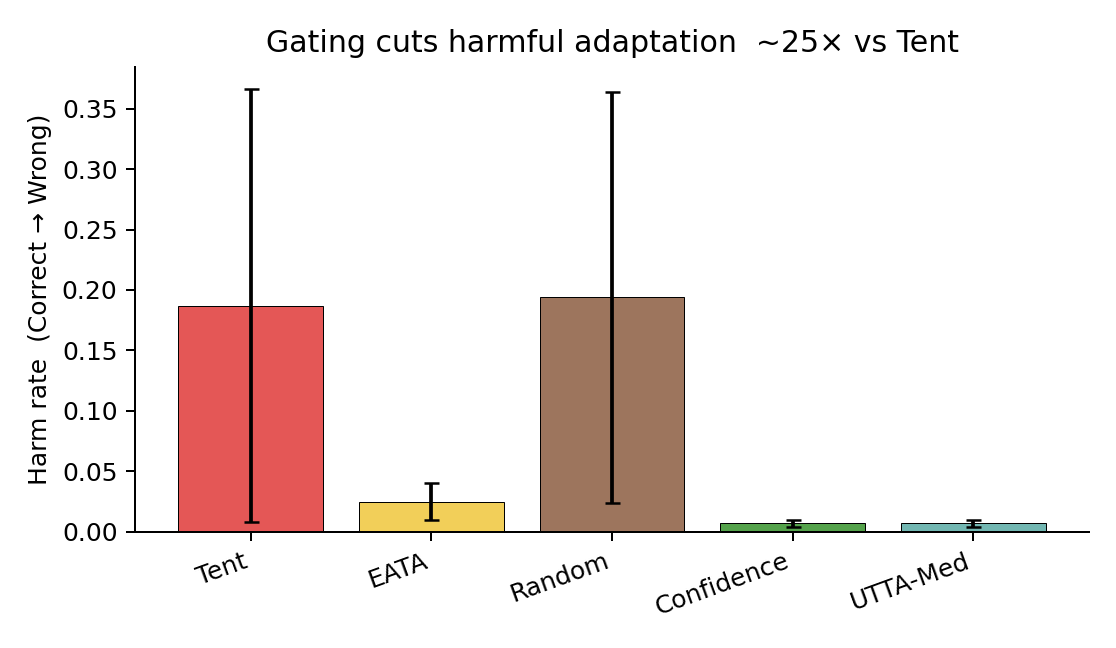
\includegraphics[width=\columnwidth]{figs/fig_harm.png}
\caption{Harm rate. Gating cuts harmful flips $\sim$25$\times$ vs.\ Tent. Random gating does not.}
\label{fig:harm}
\end{figure}

\subsection{RQ5: F1 is the clean win; ECE is not}
Gated TTA improves F1 vs.\ source on \textbf{all five seeds} (mean $+0.024$).
AUROC improves on $3/5$ seeds and is slightly below source on the two collapse-prone seeds.
ECE is not a win vs.\ source ($0.130$ vs.\ $0.128$); it \emph{is} a win vs.\ collapsing Tent.
Reliability here is primarily harm and F1, not calibration.

\subsection{RQ6: UTTA-Med $\approx$ confidence}
$|\mathrm{AUROC}_{\mathrm{UTTA}}-\mathrm{AUROC}_{\mathrm{conf}}|<0.001$ on every seed.
Entropy $\equiv$ confidence, as predicted for binary outputs.
A cheap confidence gate captures essentially all of the benefit of MC-Dropout variance for this backbone and task.
UTTA-Med remains a valid instantiation of uncertainty-gated TTA; it is not an accuracy champion over confidence.

Test coverage of confidence / entropy / UTTA is $\approx 0.51$--$0.65$, below the hospital-1 matched value $0.70$, because hospital~2 is more uncertain.
Random was run at the val-matched $0.70$ and is therefore not coverage-matched \emph{on test}.
We report both numbers.

\subsection{RQ7: Grad-CAM audit}
Grad-CAM~\cite{selvaraju2017gradcam} on the last residual stage of the seed-42 source model, $512$ shuffled hospital-2 patches (215 TP, 226 TN, 15 FP, 56 FN).
This is an interpretability audit, not clinical validation; $96\times96$ maps are coarse (Fig.~\ref{fig:cam}).

Low-uncertainty correct tumors ($p=1$, $U\sim 10^{-15}$) place CAM on dense nuclei.
Confident normals (fat/stroma) often yield \emph{blank} maps: expected for a one-logit head when the logit is strongly negative.
High-uncertainty errors sit near $p=0.5$ with edge-heavy CAMs---the population the gate excludes.
Residual failure modes that a hard gate cannot block: false positives on lymphocyte-dense tissue with $p>0.96$, and confident false negatives with $p\approx 0.01$.

\begin{figure*}[t]
\centering
\begin{minipage}{0.48\textwidth}
\centering
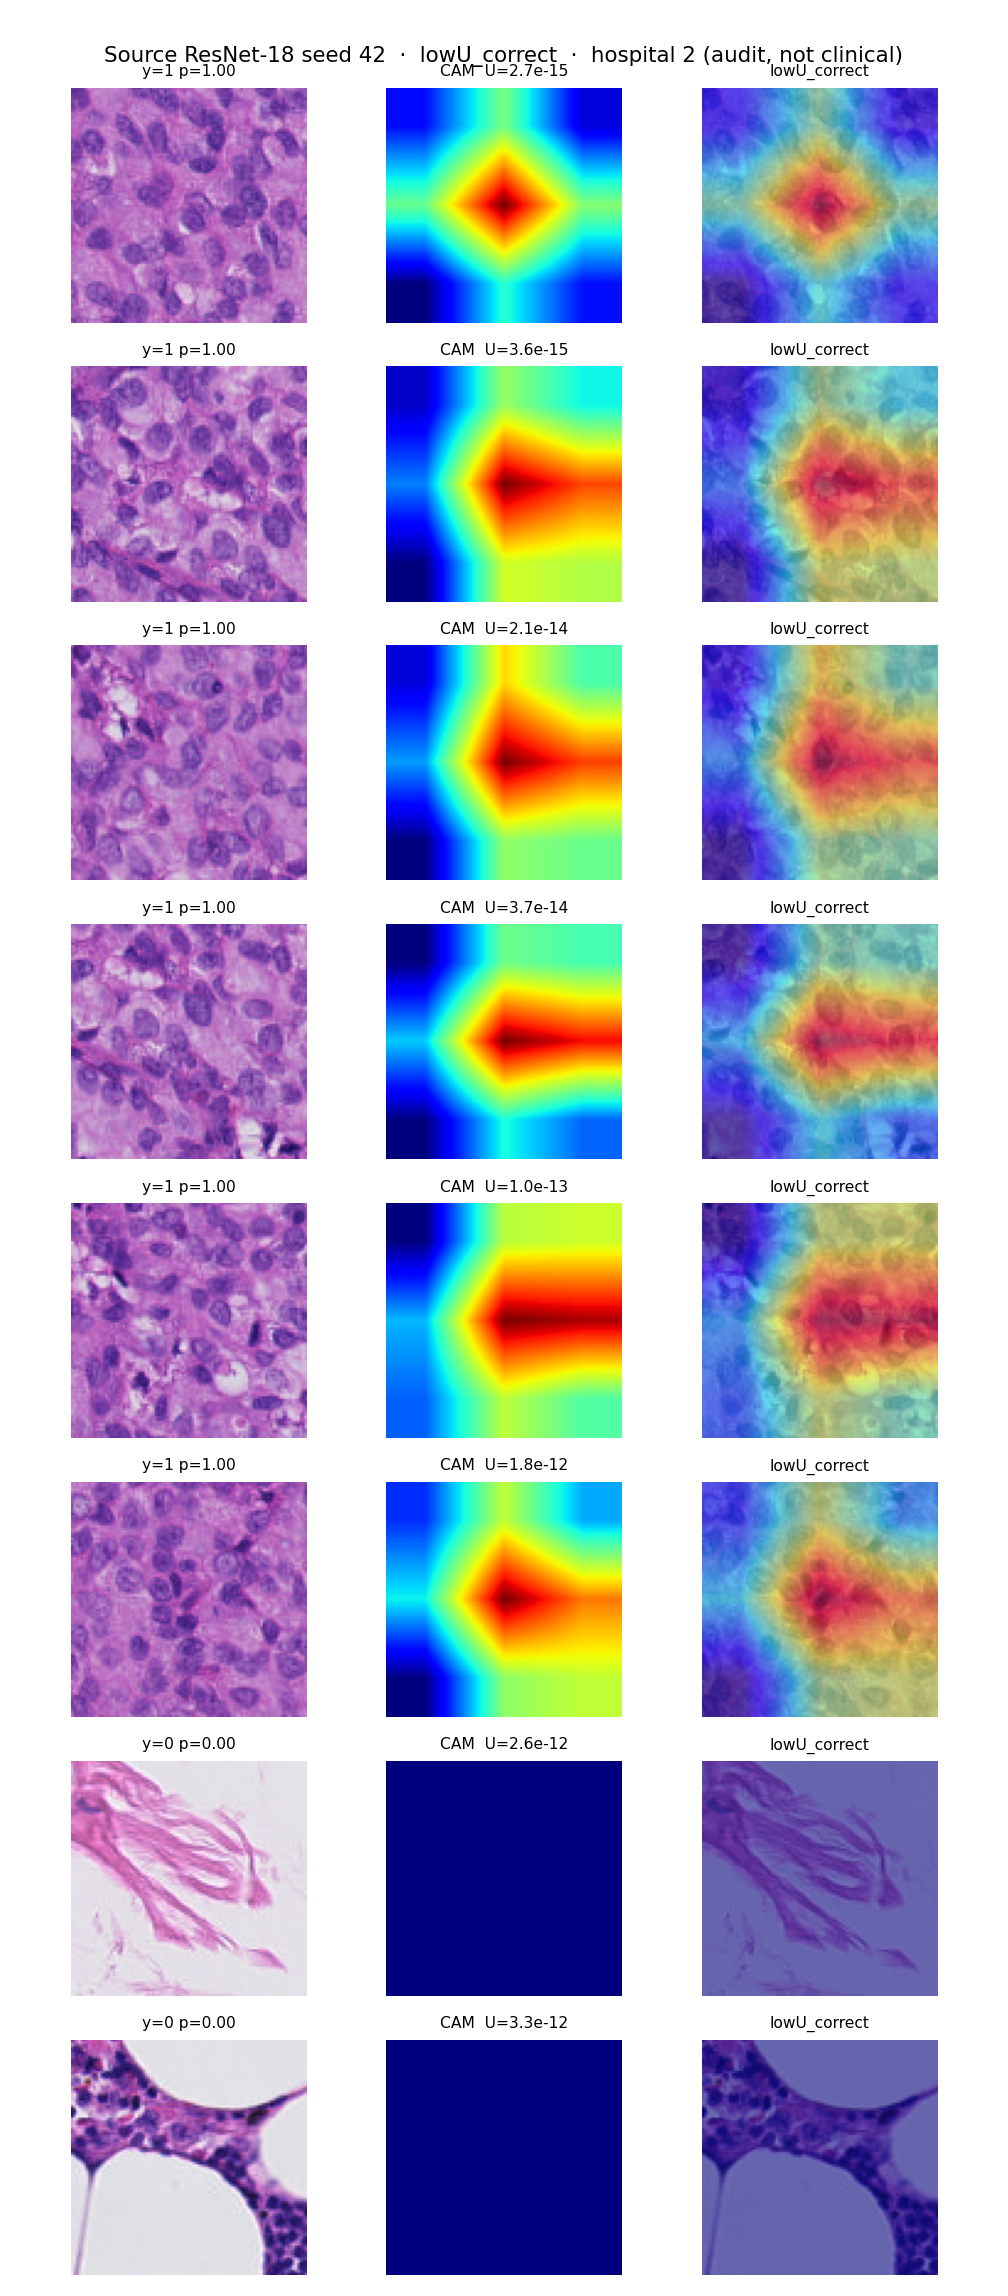
\includegraphics[width=\linewidth]{figs/fig_cam_lowu.png}\\
{\scriptsize (a) Low-$U$ correct}
\end{minipage}\hfill
\begin{minipage}{0.48\textwidth}
\centering
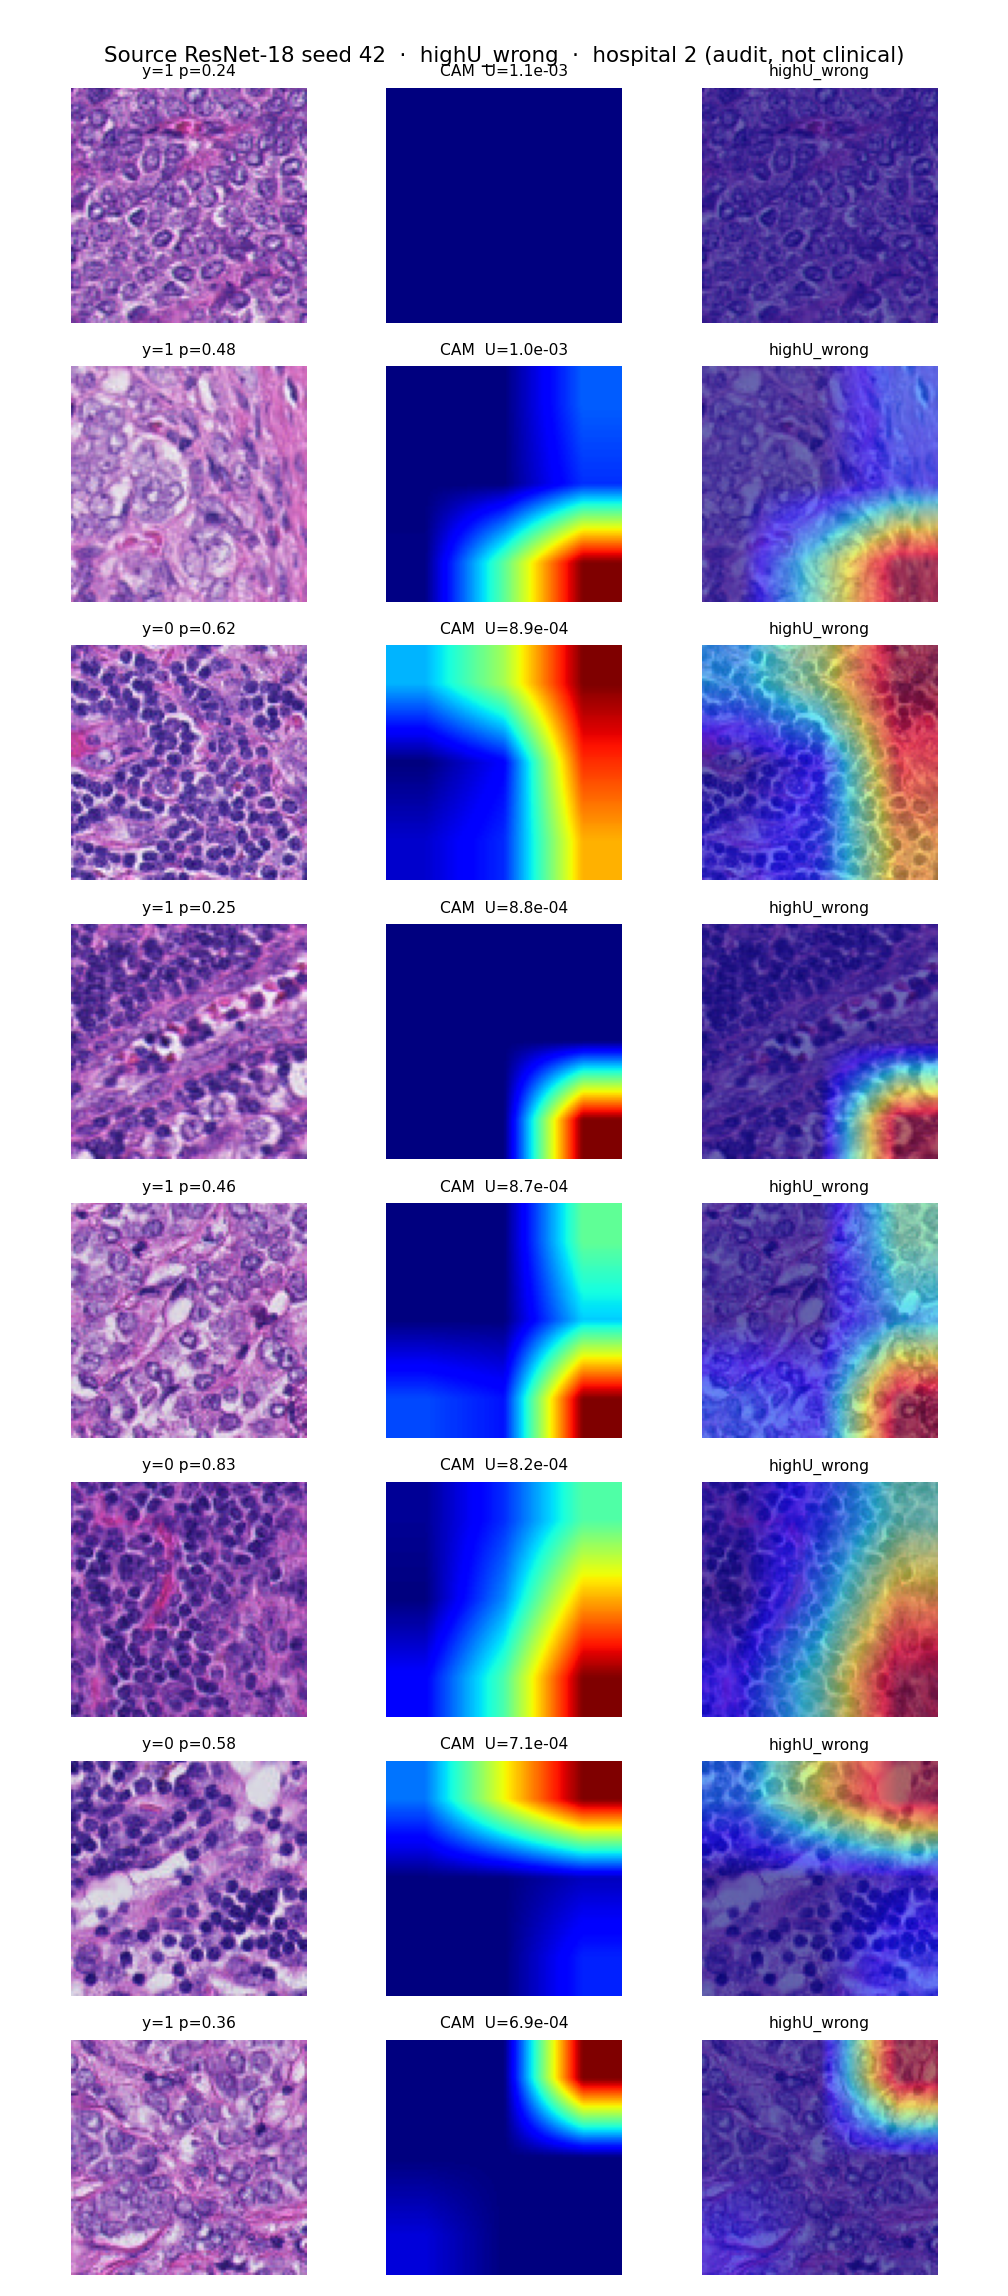
\includegraphics[width=\linewidth]{figs/fig_cam_highu.png}\\
{\scriptsize (b) High-$U$ wrong}
\end{minipage}
\caption{Grad-CAM, seed-42 source, hospital~2 (audit, not clinical validation).
(a)~Confident correct tumors attend to nuclei; confident normals often blank.
(b)~Uncertain errors near $p=0.5$ with edge CAMs---samples skipped by UTTA-Med.
Blank maps on confident negatives are a one-logit Grad-CAM artifact.}
\label{fig:cam}
\end{figure*}

\section{Discussion}

The positive statement is: under real hospital shift, unrestricted entropy-minimization TTA is unsafe, and restricting updates to high-confidence / low-variance samples makes it safe and improves F1.

The honest qualifier is: the particular Bayesian estimator (MC-Dropout variance) did not beat a softmax-confidence gate.
For a binary, well-trained ResNet, predictive variance and $|p-0.5|$ rank samples similarly.
A reviewer who knows EATA will look for this comparison; it is in Table~\ref{tab:main}.

\textbf{Limitations.}
(i)~One dataset, one backbone, binary labels.
(ii)~Reported intervals are seed-level; a WSI-level bootstrap (10 test slides) needs per-patch dumps we did not freeze in the headline JSON.
(iii)~Grad-CAM is source-only (no post-TTA pair) and blanks on confident negatives.
(iv)~Test coverage of the learned gates is below the val-matched $0.70$.
(v)~Tent's learning rate was selected on hospital~1 after larger rates collapsed; this is not Tent's original ImageNet hyperparameter.
(vi)~Confident errors still pass a hard gate.

\section{Conclusion}

Uncertainty-aware \emph{selection} makes TTA reliable on Camelyon17-WILDS; unrestricted Tent does not.
MC-Dropout is a legitimate gate, but not a better one than confidence here.
The result is worth publishing if it is written that way: a leakage-controlled reliability profile, not a forced state-of-the-art claim.

\section*{Reproducibility}
Splits: official WILDS / HF \texttt{wltjr1007/Camelyon17-WILDS}, filtered by \texttt{center}.
Seeds: $42,123,2024,7,99$.
Checkpoints: \texttt{camelyon17\_resnet18\_source\_s\{seed\}\_BEST.pt}.
Protocol: \texttt{bn\_freeze\_stats}, TTA lr $10^{-5}$, $N_{\mathrm{MC}}=20$, $\tau=$ val 70th percentile of $U$.
Every headline number traces to \texttt{camelyon17\_resnet18\_full\_s\{seed\}.json}.
Code will be released with the camera-ready.

\begin{thebibliography}{00}
\bibitem{wang2021tent} D.~Wang, E.~Shelhamer, S.~Liu, B.~Olshausen, and T.~Darrell, ``Tent: Fully test-time adaptation by entropy minimization,'' in \emph{ICLR}, 2021.
\bibitem{niu2022eata} S.~Niu, J.~Wu, Y.~Zhang, Y.~Chen, S.~Zheng, P.~Zhao, and M.~Tan, ``Efficient test-time model adaptation without forgetting,'' in \emph{ICLR}, 2022.
\bibitem{niu2023sar} S.~Niu, J.~Wu, Y.~Zhang, Z.~Wen, Y.~Chen, P.~Zhao, and M.~Tan, ``Towards stable test-time adaptation in dynamic wild world,'' in \emph{ICLR}, 2023.
\bibitem{koh2021wilds} P.~W.~Koh \emph{et al.}, ``WILDS: A benchmark of in-the-wild distribution shifts,'' in \emph{ICML}, 2021.
\bibitem{bandi2018camelyon17} P.~Bandi \emph{et al.}, ``From detection of individual metastases to classification of lymph node status at the patient level: the CAMELYON17 challenge,'' \emph{IEEE Trans.\ Med.\ Imaging}, 2019.
\bibitem{gal2016dropout} Y.~Gal and Z.~Ghahramani, ``Dropout as a Bayesian approximation: Representing model uncertainty in deep learning,'' in \emph{ICML}, 2016.
\bibitem{he2016resnet} K.~He, X.~Zhang, S.~Ren, and J.~Sun, ``Deep residual learning for image recognition,'' in \emph{CVPR}, 2016.
\bibitem{selvaraju2017gradcam} R.~R.~Selvaraju \emph{et al.}, ``Grad-CAM: Visual explanations from deep networks via gradient-based localization,'' in \emph{ICCV}, 2017.
\end{thebibliography}

\end{document}
